\documentclass[article,12pt,onesidea,4paper,english,brazil]{abntex2}

\usepackage{lmodern, indentfirst, nomencl, color, graphicx, microtype, lipsum}			
\usepackage[T1]{fontenc}		
\usepackage[utf8]{inputenc}		

\setlrmarginsandblock{2cm}{2cm}{*}
\setulmarginsandblock{2cm}{2cm}{*}
\checkandfixthelayout

\setlength{\parindent}{1.3cm}
\setlength{\parskip}{0.2cm}

\SingleSpacing

\begin{document}
	
	\selectlanguage{brazil}
	
	\frenchspacing 
	
	\begin{center}
		\LARGE ENSINO E APRENDIZAGEM EM FÍSICA UTILIZANDO O GOOGLE SKETCHUP PHYSICS 
		
		\normalsize
		Matheus Felipe de Souza e Silva\footnote{Bolsista (IC-ET), matheusfelipiss14@hotmail.com, IFRO/Campus Cacoal} 
		Gabriel Pereira da Silva\footnote{Bolsista (IC-ET), gabrielpsilva1@hotmail.com, IFRO/Campus Cacoal.} 
		Caio Afonso Côgo Oliveira\footnote{Bolsista (ICJ), caio\_cogo@hotmail.com, IFRO/Campus Cacoal} 
	Natã da Silva Stedile\footnote{Bolsista (ICJ), nata\_stedile@hotmail.com, IFRO/Campus Cacoal} 
	Átila Bezerra de Mira\footnote{Bolsista (ICJ), atilaabm4@gmail.com, IFRO/Campus Cacoal.}
	Juliano Alves de Deus\footnote{Orientador(a), juliano.alves@ifro.edu.br, IFRO/Campus Cacoal}
	\end{center}
	
	% resumo em português
	\begin{resumoumacoluna}
		Este projeto propõe utilizar a modelagem e a simulação computacional como ferramentas para a aprendizagem em física, modelando computacionalmente objetos e simulando interações físicas entre eles e com o ambiente virtual no qual estão inseridos. As modelagens e simulações computacionais foram realizadas por meio do software\textit{ Google SketchUp 8.0}, juntamente com o auxílio do\textit{ plug-in SketchPhysics 3.1}. Os experimentos realizados se mostraram compatíveis com os conceitos físicos simulados, como o equilíbrio de corpos rígidos, Leis de Newton, movimento uniformemente variado, dissipação e transferência de energia, entre outros. Estas simulações podem servir de grande auxílio para professores e alunos  e física e áreasafins.
		
		\vspace{\onelineskip}
		
		\noindent
		\textbf{Palavras-chave}: Modelagem. Simulação. SketchUp.
	\end{resumoumacoluna}
	
	\section*{Introdução}
	
	A física é uma ciência de vital importância no desenvolvimento do conhecimento humano, e seu caráter experimental é importante na comprovação e aplicação da teoria científica. Contudo, a experimentação demanda um grande aparato material, financeiro e de pessoal, muitas vezes não disponível nas instituições de ensino do Brasil. Diante disso, a modelagem e a simulação computacional surgem como alternativas para demonstrar situações físicas que se tornariam inviáveis experimentalmente. Este projeto propõe utilizar a modelagem e a simulação computacional como ferramentas para a criação de ambientes virtuais de aprendizagem em física, modelando computacionalmente objetos e simulando interações físicas entre eles e com o ambiente virtual no qual estão inseridos. Desta forma, contribuem com a atividade docente em física por meio do desenvolvimento de uma metodologia viável, inovadora e eficiente de ensino; e com o estudante por meio de um ambiente de aprendizagem estimulante, “palpável” e acessível.
	
	\section*{Material e Método}
	
A pesquisa foi desenvolvida no Laboratório de Informática do Instituto Federal de Educação, Ciência e Tecnologia/IFRO, Campus Cacoal, também sendo usados laptops pessoais. O software utilizado para a modelagem tridimensional foi o\textit{ Google SketchUp} (SKETCHUP, 2015) em sua versão gratuita 8.0 ou superior; adicionalmente, foi instalado o\textit{ plug-in SketchyPhysics} (SKETCHUCATION, 2015), versão gratuita 3.1 ou superior, que modela situações de física newtoniana. A primeira etapa foi a leitura da licença e dos manuais técnicos, a fim de entender a instalação e configuração do programa, e o estudo de tutoriais, a fim de utilizar as funções de modelagem do software. Em seguida, partiu-se para o desenvolvimento de ambientes virtuais. As modelagens e simulações foram desenvolvidas de modo a cobrir situações curriculares e práticas da física no ensino médio e técnico, com ênfase no estudo de corpos rígidos. Porém também se pode utilizar esta técnica para estudar casos de física de nível superior, ou mesmo matemática e engenharia, inclusive como ferramenta para capacitação de professores.
	\section*{Resultados e Discussão}
	
Entre os resultados obtidos por meio desta pesquisa podemos destacar as simulações que demonstraram dinamicamente diversos conceitos físicos, muitas vezes complexos e difíceis de serem representados teórica ou experimentalmente, mas que realizados em uma simulação virtual permitiram uma compreensão mais simples e “visual”. 

Assim, começamos exemplificando o equilíbrio de diferentes corpos rígidos (Figura 1). Apoiando o corpo no seu centro de massa é possível equilibrá-los, uma vez que nenhuma desproporção geométrica desequilibra o sistema; já qualquer alteração na posição deste apoio provoca o desequilíbrio e a queda do corpo (NUSSENZVEIG, H. M., 2002), mostrando que o software reflete de forma bastante fiel o conceito teórico.
\begin{figure}[h]
	\centering
	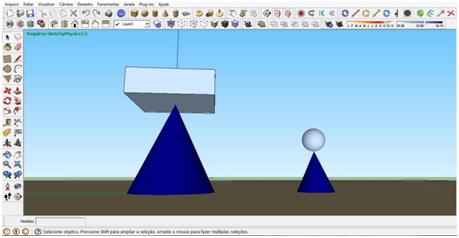
\includegraphics[width=0.7\linewidth]{pip-pg70-01}
	\caption{Equilíbriodecorposrígidos,apoiadosnoseucentrodemassa.Qualqueralteraçãona posiçãodeapoioprovocaaquedadocorporígido}
	\label{fig:pip-pg70-01}
\end{figure}

Outro exemplo bem representado virtualmente é o movimento uniformemente variado, M.U.V. (Figura 2). Neste caso foi testada a aceleração de três esferas caindo sobre rampas. Mesmo o software não tendo uma opção de marcação de tempo, foi possível, por meio da visualização ou de um cronômetro externo, observar a maior aceleração desses corpos de acordo com a inclinação de suas respectivas rampas. Foi possível inclusive ajustar o comprimento das rampas para que as esferas chegassem ao mesmo tempo no nível mais baixo, mostrando assim que o software modela de forma satisfatória as equações doM.U.V.
\begin{figure}[h]
	\centering
	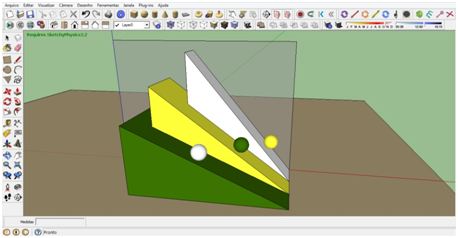
\includegraphics[width=0.5\linewidth]{pip-pg70-02}
	\caption{Movimento uniformemente variado de esferas sobre rampas}
	\label{fig:pip-pg70-02}
\end{figure}

Foram realizadas também outras simulações que se mostraram bem representadas pelo software e que podem servir de base para demonstrações práticas em física, como a colisão de partículas e a Terceira Lei de Newton (Figura
3)	e a transferência de energia num pulso (Figura 4), entreoutras. 
\begin{figure}[h]
	\centering
	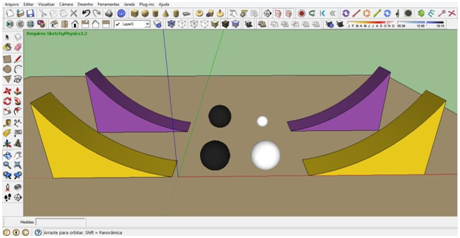
\includegraphics[width=0.5\linewidth]{pip-pg70-03}
	\caption{Terceira Lei de Newton (ação e reação) numa colisão de esferas.}
	\label{fig:pip-pg70-03}
\end{figure}

\begin{figure}[h]
	\centering
	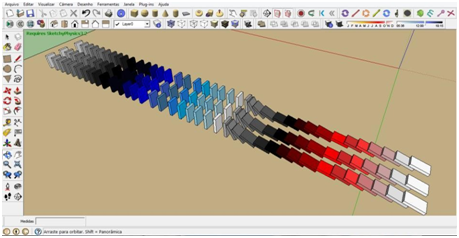
\includegraphics[width=0.5\linewidth]{pip-pg70-04}
	\caption{: Transferência de energia em efeito dominó}
	\label{fig:pip-pg70-04}
\end{figure}

	
	\section*{Conclusões}
	
	Podemos concluir por meio destes exemplos que o software \textit{SketchUp}, juntamente com o \textit{  plug-in SketchPhysics}, são capazes de modelar e simular de forma satisfatória muitas situações físicas envolvendo corpos rígidos. Assim, é possível simular computacionalmente experimentos físicos que, por meio de um laboratório,demandariamumgrandeinvestimentofinanceiro,tecnológicoede pessoal, mas que de forma virtual podem ser realizados na tela do computador dos discentes, o que torna o método bastante viável. Cite-se, no entanto, que a proposta deste trabalho não é substituir a experimentação pela simulação, mas sim desenvolver uma metodologia de ensino viável para a materialização dos conceitos teóricos quando a experimentação é indisponível ou improdutiva.
	
	Assim, a modelagem e a simulação contribuem com a atividade do docente em física por meio do desenvolvimento de uma metodologia inovadora e eficiente de ensino; e com o estudante por meio de um ambiente de aprendizagem estimulante, acessível e “palpável”.
	\section*{agradecimento}
	
	Agradecemos ao IFRO, à PROPESP e à FAPERO pelo apoio logístico, material e financeiro para o desenvolvimento desta pesquisa.
	\section*{Instituição de Fomento}
	
Departamento de Pesquisa, Inovação e Pós-Gradução – IFRO/Campus Cacoal. Pró-Reitoria de Pesquisa, Inovação e Pós-Gradução – IFRO.
\\Fundação de Amparo ao Desenvolvimento das Ações Científicas e tecnológicas e à Pesquisa – FAPERO.

	
	\section*{Referências}
		\noindent NUSSENZVEIG, H. M. Curso de física básica. 4. ed. v. 1-4. São Paulo: Edgard Blucher LTDA, 2002.
		
	\noindent	SKETCHUCATION.	Disponível	em:
		<http:sketchucation.com/pluginstore?pln=ScketchyPhysics>. Último acesso em: 22 de set. 2016.
		
	\noindent	SKETCHUP. The easiest way to draw in 3D. Disponível em: <http://www.sketchup.com/pt- BR>. Último acesso em: 22 set. 2016.

\end{document}